% Options for packages loaded elsewhere
\PassOptionsToPackage{unicode}{hyperref}
\PassOptionsToPackage{hyphens}{url}
%
\documentclass[
]{article}
\usepackage{amsmath,amssymb}
\usepackage{lmodern}
\usepackage{ifxetex,ifluatex}
\ifnum 0\ifxetex 1\fi\ifluatex 1\fi=0 % if pdftex
  \usepackage[T1]{fontenc}
  \usepackage[utf8]{inputenc}
  \usepackage{textcomp} % provide euro and other symbols
\else % if luatex or xetex
  \usepackage{unicode-math}
  \defaultfontfeatures{Scale=MatchLowercase}
  \defaultfontfeatures[\rmfamily]{Ligatures=TeX,Scale=1}
\fi
% Use upquote if available, for straight quotes in verbatim environments
\IfFileExists{upquote.sty}{\usepackage{upquote}}{}
\IfFileExists{microtype.sty}{% use microtype if available
  \usepackage[]{microtype}
  \UseMicrotypeSet[protrusion]{basicmath} % disable protrusion for tt fonts
}{}
\makeatletter
\@ifundefined{KOMAClassName}{% if non-KOMA class
  \IfFileExists{parskip.sty}{%
    \usepackage{parskip}
  }{% else
    \setlength{\parindent}{0pt}
    \setlength{\parskip}{6pt plus 2pt minus 1pt}}
}{% if KOMA class
  \KOMAoptions{parskip=half}}
\makeatother
\usepackage{xcolor}
\IfFileExists{xurl.sty}{\usepackage{xurl}}{} % add URL line breaks if available
\IfFileExists{bookmark.sty}{\usepackage{bookmark}}{\usepackage{hyperref}}
\hypersetup{
  pdftitle={Data Envelopment Analysis (DEA)},
  pdfauthor={Muthia Salsabila},
  hidelinks,
  pdfcreator={LaTeX via pandoc}}
\urlstyle{same} % disable monospaced font for URLs
\usepackage[margin=1in]{geometry}
\usepackage{color}
\usepackage{fancyvrb}
\newcommand{\VerbBar}{|}
\newcommand{\VERB}{\Verb[commandchars=\\\{\}]}
\DefineVerbatimEnvironment{Highlighting}{Verbatim}{commandchars=\\\{\}}
% Add ',fontsize=\small' for more characters per line
\usepackage{framed}
\definecolor{shadecolor}{RGB}{248,248,248}
\newenvironment{Shaded}{\begin{snugshade}}{\end{snugshade}}
\newcommand{\AlertTok}[1]{\textcolor[rgb]{0.94,0.16,0.16}{#1}}
\newcommand{\AnnotationTok}[1]{\textcolor[rgb]{0.56,0.35,0.01}{\textbf{\textit{#1}}}}
\newcommand{\AttributeTok}[1]{\textcolor[rgb]{0.77,0.63,0.00}{#1}}
\newcommand{\BaseNTok}[1]{\textcolor[rgb]{0.00,0.00,0.81}{#1}}
\newcommand{\BuiltInTok}[1]{#1}
\newcommand{\CharTok}[1]{\textcolor[rgb]{0.31,0.60,0.02}{#1}}
\newcommand{\CommentTok}[1]{\textcolor[rgb]{0.56,0.35,0.01}{\textit{#1}}}
\newcommand{\CommentVarTok}[1]{\textcolor[rgb]{0.56,0.35,0.01}{\textbf{\textit{#1}}}}
\newcommand{\ConstantTok}[1]{\textcolor[rgb]{0.00,0.00,0.00}{#1}}
\newcommand{\ControlFlowTok}[1]{\textcolor[rgb]{0.13,0.29,0.53}{\textbf{#1}}}
\newcommand{\DataTypeTok}[1]{\textcolor[rgb]{0.13,0.29,0.53}{#1}}
\newcommand{\DecValTok}[1]{\textcolor[rgb]{0.00,0.00,0.81}{#1}}
\newcommand{\DocumentationTok}[1]{\textcolor[rgb]{0.56,0.35,0.01}{\textbf{\textit{#1}}}}
\newcommand{\ErrorTok}[1]{\textcolor[rgb]{0.64,0.00,0.00}{\textbf{#1}}}
\newcommand{\ExtensionTok}[1]{#1}
\newcommand{\FloatTok}[1]{\textcolor[rgb]{0.00,0.00,0.81}{#1}}
\newcommand{\FunctionTok}[1]{\textcolor[rgb]{0.00,0.00,0.00}{#1}}
\newcommand{\ImportTok}[1]{#1}
\newcommand{\InformationTok}[1]{\textcolor[rgb]{0.56,0.35,0.01}{\textbf{\textit{#1}}}}
\newcommand{\KeywordTok}[1]{\textcolor[rgb]{0.13,0.29,0.53}{\textbf{#1}}}
\newcommand{\NormalTok}[1]{#1}
\newcommand{\OperatorTok}[1]{\textcolor[rgb]{0.81,0.36,0.00}{\textbf{#1}}}
\newcommand{\OtherTok}[1]{\textcolor[rgb]{0.56,0.35,0.01}{#1}}
\newcommand{\PreprocessorTok}[1]{\textcolor[rgb]{0.56,0.35,0.01}{\textit{#1}}}
\newcommand{\RegionMarkerTok}[1]{#1}
\newcommand{\SpecialCharTok}[1]{\textcolor[rgb]{0.00,0.00,0.00}{#1}}
\newcommand{\SpecialStringTok}[1]{\textcolor[rgb]{0.31,0.60,0.02}{#1}}
\newcommand{\StringTok}[1]{\textcolor[rgb]{0.31,0.60,0.02}{#1}}
\newcommand{\VariableTok}[1]{\textcolor[rgb]{0.00,0.00,0.00}{#1}}
\newcommand{\VerbatimStringTok}[1]{\textcolor[rgb]{0.31,0.60,0.02}{#1}}
\newcommand{\WarningTok}[1]{\textcolor[rgb]{0.56,0.35,0.01}{\textbf{\textit{#1}}}}
\usepackage{graphicx}
\makeatletter
\def\maxwidth{\ifdim\Gin@nat@width>\linewidth\linewidth\else\Gin@nat@width\fi}
\def\maxheight{\ifdim\Gin@nat@height>\textheight\textheight\else\Gin@nat@height\fi}
\makeatother
% Scale images if necessary, so that they will not overflow the page
% margins by default, and it is still possible to overwrite the defaults
% using explicit options in \includegraphics[width, height, ...]{}
\setkeys{Gin}{width=\maxwidth,height=\maxheight,keepaspectratio}
% Set default figure placement to htbp
\makeatletter
\def\fps@figure{htbp}
\makeatother
\setlength{\emergencystretch}{3em} % prevent overfull lines
\providecommand{\tightlist}{%
  \setlength{\itemsep}{0pt}\setlength{\parskip}{0pt}}
\setcounter{secnumdepth}{-\maxdimen} % remove section numbering
\ifluatex
  \usepackage{selnolig}  % disable illegal ligatures
\fi

\title{Data Envelopment Analysis (DEA)}
\author{Muthia Salsabila}
\date{}

\begin{document}
\maketitle

This Notebook show how to estimate and measure efficiency using Data
Envelopment Analysis (DEA) method and Benchmarking package in R.

What is Efficiency?\\
Efficiency is when a firm can minimize its input to produce a particular
output. There are three types of efficiency, which are technical
efficiency, allocative efficiency, and economic efficiency. Technical
efficiency is a firm ability to reach optimal output using a particular
input. Allocative efficiency is a firm ability to use optimal input to
reach a certain level of output. Economic efficiency is a combination
between technical efficiency and allocative efficiency.

Efficiency can be measure with DEA and SFA. We will be using DEA method
for measuring the efficiency.

What is Data Envelopment Analysis?\\
Data Envelopment Analysis (DEA) is a non-parametric linear programming
approach for measuring efficiency that can measure multiple-input and
multiple-output. DEA introduced by Charnes, Coopers, and Rhodes in 1978.

There are two assumptions in DEA, which are Constant Return to Scale
(CRS) and Variable Return to Scale (VRS).\\

CRS assume a firm operate at optimum scale and the ratio of increasing
input is equal to output, which mean if there is an addition to input x
times then the output will increase x times too. CRS model often define
as CCR model because it introduced by Charnes, Cooper, and Rhodes.

VRS (or known as BCC model, developed by Banker, Charnes, and Cooper)
assume a firm not or not yet operate at optimum scale and the ratio
between input and ouput is not equal. When there is an addition to input
x times, the output can increase more than x or lower than x.

There's also two approach in DEA:

Input oriented = minimizing input to reach a certain level of output

output oriented = maximizing output using a particular combination of
input

Step of Project\\
1. Loading Packages\\
2. Import Data\\
3. Select Input and Output\\
4. Estimate Efficiencies\\
5. Measure Slack\\
6. Plot Frontier

Loading Packages\\
The first step is to load the Benchmarking package using library
function. This package contains methods to estimate and measure
efficiency using DEA and SFA.

\begin{Shaded}
\begin{Highlighting}[]
\FunctionTok{library}\NormalTok{(Benchmarking)}
\end{Highlighting}
\end{Shaded}

Import data\\
This package also contains a few datasets that can be used for practice.
The datasets I use called \emph{milkProd}, which is a data from Danish
milk producers. I also use dplyr package to see a glimpse of data rows,
column, and type.

\begin{Shaded}
\begin{Highlighting}[]
\CommentTok{\#import data}
\FunctionTok{data}\NormalTok{(}\StringTok{"milkProd"}\NormalTok{)}
\NormalTok{milkProd}
\end{Highlighting}
\end{Shaded}

\begin{verbatim}
##     farmNo    milk energy    vet cows
## 1        1  862533 117894  21186  121
## 2        2  605764  72049  43910   80
## 3        3  865658 158466  54583   95
## 4        4  662331  66783  45469   87
## 5        5 1003444 101714  81625  125
## 6        6  923512 252408  96807  135
## 7        7  563685 131025  51901   87
## 8        8 1247312 154591  38164  171
## 9        9  992729 187575  82810  165
## 10      10 1209692 251479  72818  154
## 11      11  575313  71678  43034   79
## 12      12  494145 123044  13743   99
## 13      13  962390 188050  51897  107
## 14      14  889904 160004  50729  111
## 15      15 1493202 335961  40479  196
## 16      16 1041920 123878  62653  133
## 17      17  529246  96749  48489   79
## 18      18 1153076 110201  91842  132
## 19      19  655203  95837  73460   93
## 20      20  722228 107473  44058   96
## 21      21 1237837 216102  81282  155
## 22      22  935153 146657  70010  120
## 23      23  851469 219861  25179  154
## 24      24  751310  86185  71552   91
## 25      25  597157  84704  30057   86
## 26      26  651113  97623  46495   88
## 27      27  945643  75221 120521  155
## 28      28 1510578 132574  67460  186
## 29      29  163413  12977   6390   25
## 30      30  887097 108778  67646  121
## 31      31 1593729 295293  27419  208
## 32      32 1149521 177074  65327  141
## 33      33  989964  87601  34990  146
## 34      34 1049369 129586  31427  113
## 35      35  261795  68490  22821   52
## 36      36  557805 103485  30000   80
## 37      37  364975  56276  25086   54
## 38      38  683575 121530  31662   96
## 39      39  543277  76820  45130   82
## 40      40  744681  50116  44894  106
## 41      41  139625  35400   4421   34
## 42      42  751292 112151  59460  105
## 43      43 1247409 204472  86450  169
## 44      44 1101321 124452  89135  149
## 45      45  702507 117935  68007   92
## 46      46  731246 155390  56664  137
## 47      47  611823  68801 103226   79
## 48      48  554570 106841  65929   77
## 49      49  483198  66999  17102   69
## 50      50  986515 141035 116905  115
## 51      51  873100 113294  61777  111
## 52      52  523624 111243   7548   69
## 53      53  125574  24570  10521   21
## 54      54  801977 137498  55470  110
## 55      55  503982  77989  55015   97
## 56      56 1144855 205242  58282  164
## 57      57  868317 126092  44166  127
## 58      58  348958  66228   7156   44
## 59      59  408782  59263   7721   61
## 60      60  855654  97964 107462  110
## 61      61  877160 174860  64943  105
## 62      62  997954 137021  76767  132
## 63      63 1120067 193124  75860  135
## 64      64  894082 107865  65704  111
## 65      65  406904  99075  19160   79
## 66      66  791920  97377  48291   88
## 67      67  529967  62740  35413   82
## 68      68  608970 123999  79464   82
## 69      69  926933 126548  69051  113
## 70      70  661690 161899  53260   88
## 71      71  354532  54682  37420   48
## 72      72  564456 102271  59124   71
## 73      73  965119 165220  29770  114
## 74      74  996852 138487  81515  135
## 75      75  493540  97523  26028   80
## 76      76  659716  80353  45669   94
## 77      77  559728  78590  44483   70
## 78      78  465213  66506  47319   74
## 79      79  891886 128964  51573  109
## 80      80  573431  93166  23293   90
## 81      81  867275  84425  72895  101
## 82      82  973988 145678  77904  111
## 83      83  578494  85415  13969   66
## 84      84  636342 137193  20353   78
## 85      85  282491  61701   9712   49
## 86      86  361620  58554  14272   74
## 87      87  963544 234715 109654  194
## 88      88  750463  73797  32496  109
## 89      89  433043  94296  44851   58
## 90      90  799765 111386  21374  105
## 91      91  178039  14582  27058   34
## 92      92  823233 134097  70874  152
## 93      93 1048629 129644  95131  115
## 94      94  730206 115743  50786   88
## 95      95 1068747 163608  68044  140
## 96      96  958127 190158  83585  116
## 97      97 1180026 124998  58576  157
## 98      98  627704 117625  74905  110
## 99      99  512459  56162  40291   64
## 100    100  569737  47471  44808   72
## 101    101  393383  59946  32418   52
## 102    102  413086  30397  18053   71
## 103    103  441835  73450  35536   61
## 104    104  342816  56077  18511   45
## 105    105 1047603  75114  73498  126
## 106    106  894828 142008  66516  116
## 107    107  983645 190440  73142  116
## 108    108  738916 156109 115209   92
\end{verbatim}

\begin{Shaded}
\begin{Highlighting}[]
\NormalTok{dplyr}\SpecialCharTok{::}\FunctionTok{glimpse}\NormalTok{(milkProd)}
\end{Highlighting}
\end{Shaded}

\begin{verbatim}
## Rows: 108
## Columns: 5
## $ farmNo <int> 1, 2, 3, 4, 5, 6, 7, 8, 9, 10, 11, 12, 13, 14, 15, 16, 17, 18, ~
## $ milk   <int> 862533, 605764, 865658, 662331, 1003444, 923512, 563685, 124731~
## $ energy <int> 117894, 72049, 158466, 66783, 101714, 252408, 131025, 154591, 1~
## $ vet    <int> 21186, 43910, 54583, 45469, 81625, 96807, 51901, 38164, 82810, ~
## $ cows   <int> 121, 80, 95, 87, 125, 135, 87, 171, 165, 154, 79, 99, 107, 111,~
\end{verbatim}

As we can see, the data has 108 rows and 5 columns with all variables
data type are integer. The variable name meaning are as follows:

\begin{itemize}
\tightlist
\item
  \textbf{farmNO} = farm number\\
\item
  \textbf{milk} = Output of milk, kg\\
\item
  \textbf{energy} = Energy Expenses\\
\item
  \textbf{vet} = Veterinary expenses\\
\item
  \textbf{cows} = Number of Cows
\end{itemize}

Select Input and Output\\
To estimate the efficiency, we must select which variables from the data
are input and which are the output. DEA can select multiple output and
multiple input, but in this case we use only one output and multiple
input.

\begin{Shaded}
\begin{Highlighting}[]
\CommentTok{\# input output selection}
\NormalTok{x }\OtherTok{\textless{}{-}} \FunctionTok{with}\NormalTok{(milkProd, }\FunctionTok{cbind}\NormalTok{(energy, vet, cows))}
\NormalTok{y }\OtherTok{\textless{}{-}} \FunctionTok{with}\NormalTok{(milkProd, }\FunctionTok{cbind}\NormalTok{(milk))}
\end{Highlighting}
\end{Shaded}

X define the input variables which are energy expenses, veterinary
expenses, and number of cows. While y define the output variable which
is milk in kilogram.

Calculate Efficiency\\
After we select the input and output, we can calculate the efficiency
using dea function as follows:

\begin{Shaded}
\begin{Highlighting}[]
\CommentTok{\#calculating efficiency}
\CommentTok{\#VRS (bcc)}
\NormalTok{bcc }\OtherTok{\textless{}{-}} \FunctionTok{dea}\NormalTok{(x, y, }\AttributeTok{RTS =} \StringTok{"vrs"}\NormalTok{, }\AttributeTok{ORIENTATION =} \StringTok{"in"}\NormalTok{)}
\FunctionTok{eff}\NormalTok{(bcc)}
\end{Highlighting}
\end{Shaded}

\begin{verbatim}
##   [1] 1.0000000 0.8844248 0.9964530 0.9073615 0.9247900 0.7439829 0.7417086
##   [8] 0.9983316 0.6508284 0.8985446 0.8529547 0.6730465 0.9749370 0.8746228
##  [15] 0.9612959 0.8798740 0.7740659 1.0000000 0.7974214 0.8380647 0.9214881
##  [22] 0.8466635 0.6816404 0.9411051 0.7985195 0.8338680 0.8867200 1.0000000
##  [29] 1.0000000 0.8354960 1.0000000 0.9138441 1.0000000 1.0000000 0.6641207
##  [36] 0.7993055 0.8317462 0.7967560 0.7751629 1.0000000 1.0000000 0.7965694
##  [43] 0.8541166 0.8460606 0.8519376 0.5936892 0.9092675 0.8262730 0.8521087
##  [50] 0.9280546 0.8759278 1.0000000 1.0000000 0.8027888 0.6284807 0.7811798
##  [57] 0.7657584 1.0000000 1.0000000 0.8897330 0.9124867 0.8332759 0.9199263
##  [64] 0.9044265 0.6201782 0.9933319 0.7844554 0.8419748 0.8932946 0.8443652
##  [71] 0.9127449 0.9099331 0.9276124 0.8158349 0.7200275 0.8220379 0.9180417
##  [78] 0.7517989 0.8924859 0.7415167 0.9922742 0.9502334 1.0000000 0.9201801
##  [85] 0.7566123 0.7131812 0.5383167 0.9167356 0.8887702 0.9637106 0.9540187
##  [92] 0.6218999 0.9855879 0.9220796 0.8290510 0.8956272 0.8945004 0.6462622
##  [99] 0.9528539 0.9757119 0.9167640 1.0000000 0.8601009 0.9464849 1.0000000
## [106] 0.8411605 0.9175846 0.8914390
\end{verbatim}

We use BCC model and input-oriented.

\begin{Shaded}
\begin{Highlighting}[]
\FunctionTok{summary}\NormalTok{(bcc)}
\end{Highlighting}
\end{Shaded}

\begin{verbatim}
## Summary of efficiencies
## VRS technology and input orientated efficiency
## Number of firms with efficiency==1 are 16 out of 108 
## Mean efficiency: 0.868 
## ---                
##   Eff range       #    %
##   0.5<= E <0.6    2  1.9
##   0.6<= E <0.7    8  7.4
##   0.7<= E <0.8   17 15.7
##   0.8<= E <0.9   33 30.6
##   0.9<= E <1     32 29.6
##         E ==1    16 14.8
##    Min. 1st Qu.  Median    Mean 3rd Qu.    Max. 
##  0.5383  0.8019  0.8906  0.8681  0.9509  1.0000
\end{verbatim}

From the summary we can see there are 16 DMUs categorized as efficient,
and the mean efficiency is 0.868.

We also can see how much DMUs become a peers for other DMU. As we see
below, L34 or DMU number 34 become peers for 80 other DMUs.

\begin{Shaded}
\begin{Highlighting}[]
\FunctionTok{get.number.peers}\NormalTok{(bcc)}
\end{Highlighting}
\end{Shaded}

\begin{verbatim}
##      peer count
## L1      1     2
## L18    18     2
## L28    28    12
## L29    29    47
## L31    31     7
## L33    33     5
## L34    34    80
## L40    40     3
## L41    41     1
## L52    52     3
## L53    53    21
## L58    58     2
## L59    59     6
## L83    83    38
## L102  102     1
## L105  105    33
\end{verbatim}

Using get.which.peers function, we can see DMUs group by its peer.

\begin{Shaded}
\begin{Highlighting}[]
\FunctionTok{get.which.peers}\NormalTok{(bcc)}
\end{Highlighting}
\end{Shaded}

\begin{verbatim}
## $L1
## [1]  1 90
## 
## $L18
## [1] 18 44
## 
## $L28
##  [1]  8 10 15 21 28 32 43 56 63 88 95 97
## 
## $L29
##  [1]   2   4   5   9  11  16  19  20  24  25  26  29  30  37  39  42  46  47  49
## [20]  51  55  57  60  62  64  65  66  67  69  71  74  76  77  78  80  81  85  86
## [39]  88  91  92  93  97  98  99 100 101
## 
## $L31
## [1]  8 12 15 23 31 73 90
## 
## $L33
## [1]  8 33 49 86 88
## 
## $L34
##  [1]   2   3   4   5   6   9  10  11  13  14  15  16  17  19  20  21  22  24  25
## [20]  26  30  32  34  37  38  39  42  43  44  45  46  47  49  50  51  54  55  56
## [39]  57  60  61  62  63  64  66  67  68  69  70  71  73  74  75  76  77  78  79
## [58]  80  81  82  84  86  87  88  90  92  93  94  95  96  97  98  99 100 101 103
## [77] 104 106 107 108
## 
## $L40
## [1] 27 40 91
## 
## $L41
## [1] 41
## 
## $L52
## [1] 12 23 52
## 
## $L53
##  [1]   7  17  20  26  35  36  37  46  48  53  65  66  71  72  75  77  89  98 101
## [20] 103 104
## 
## $L58
## [1] 58 85
## 
## $L59
## [1] 12 49 59 80 86 90
## 
## $L83
##  [1]   3   6   7  12  13  14  17  22  23  35  36  38  45  48  50  54  61  65  68
## [20]  70  72  73  75  79  80  82  83  84  85  87  89  94  96 103 104 106 107 108
## 
## $L102
## [1] 102
## 
## $L105
##  [1]   2   4   5   9  11  16  19  24  25  27  30  39  42  44  47  51  55  57  60
## [20]  62  64  67  69  74  76  78  81  92  93  97  99 100 105
\end{verbatim}

While below is a list of DMU with their reference peer. DMU number 2
follow DMU 29, DMU 34, and DMU 105 as an example so DMU number 2 can be
efficient.

\begin{Shaded}
\begin{Highlighting}[]
\FunctionTok{print}\NormalTok{(}\FunctionTok{peers}\NormalTok{(bcc,}\AttributeTok{NAMES=}\ConstantTok{TRUE}\NormalTok{),}\AttributeTok{quote=}\ConstantTok{FALSE}\NormalTok{)}
\end{Highlighting}
\end{Shaded}

\begin{verbatim}
##        peer1 peer2 peer3 peer4
##   [1,] 1     <NA>  <NA>  <NA> 
##   [2,] 29    34    105   <NA> 
##   [3,] 34    83    <NA>  <NA> 
##   [4,] 29    34    105   <NA> 
##   [5,] 29    34    105   <NA> 
##   [6,] 34    83    <NA>  <NA> 
##   [7,] 53    83    <NA>  <NA> 
##   [8,] 28    31    33    <NA> 
##   [9,] 29    34    105   <NA> 
##  [10,] 28    34    <NA>  <NA> 
##  [11,] 29    34    105   <NA> 
##  [12,] 31    52    59    83   
##  [13,] 34    83    <NA>  <NA> 
##  [14,] 34    83    <NA>  <NA> 
##  [15,] 28    31    34    <NA> 
##  [16,] 29    34    105   <NA> 
##  [17,] 34    53    83    <NA> 
##  [18,] 18    <NA>  <NA>  <NA> 
##  [19,] 29    34    105   <NA> 
##  [20,] 29    34    53    <NA> 
##  [21,] 28    34    <NA>  <NA> 
##  [22,] 34    83    <NA>  <NA> 
##  [23,] 31    52    83    <NA> 
##  [24,] 29    34    105   <NA> 
##  [25,] 29    34    105   <NA> 
##  [26,] 29    34    53    <NA> 
##  [27,] 40    105   <NA>  <NA> 
##  [28,] 28    <NA>  <NA>  <NA> 
##  [29,] 29    <NA>  <NA>  <NA> 
##  [30,] 29    34    105   <NA> 
##  [31,] 31    <NA>  <NA>  <NA> 
##  [32,] 28    34    <NA>  <NA> 
##  [33,] 33    <NA>  <NA>  <NA> 
##  [34,] 34    <NA>  <NA>  <NA> 
##  [35,] 53    83    <NA>  <NA> 
##  [36,] 53    83    <NA>  <NA> 
##  [37,] 29    34    53    <NA> 
##  [38,] 34    83    <NA>  <NA> 
##  [39,] 29    34    105   <NA> 
##  [40,] 40    <NA>  <NA>  <NA> 
##  [41,] 41    <NA>  <NA>  <NA> 
##  [42,] 29    34    105   <NA> 
##  [43,] 28    34    <NA>  <NA> 
##  [44,] 18    34    105   <NA> 
##  [45,] 34    83    <NA>  <NA> 
##  [46,] 29    34    53    <NA> 
##  [47,] 29    34    105   <NA> 
##  [48,] 53    83    <NA>  <NA> 
##  [49,] 29    33    34    59   
##  [50,] 34    83    <NA>  <NA> 
##  [51,] 29    34    105   <NA> 
##  [52,] 52    <NA>  <NA>  <NA> 
##  [53,] 53    <NA>  <NA>  <NA> 
##  [54,] 34    83    <NA>  <NA> 
##  [55,] 29    34    105   <NA> 
##  [56,] 28    34    <NA>  <NA> 
##  [57,] 29    34    105   <NA> 
##  [58,] 58    <NA>  <NA>  <NA> 
##  [59,] 59    <NA>  <NA>  <NA> 
##  [60,] 29    34    105   <NA> 
##  [61,] 34    83    <NA>  <NA> 
##  [62,] 29    34    105   <NA> 
##  [63,] 28    34    <NA>  <NA> 
##  [64,] 29    34    105   <NA> 
##  [65,] 29    53    83    <NA> 
##  [66,] 29    34    53    <NA> 
##  [67,] 29    34    105   <NA> 
##  [68,] 34    83    <NA>  <NA> 
##  [69,] 29    34    105   <NA> 
##  [70,] 34    83    <NA>  <NA> 
##  [71,] 29    34    53    <NA> 
##  [72,] 53    83    <NA>  <NA> 
##  [73,] 31    34    83    <NA> 
##  [74,] 29    34    105   <NA> 
##  [75,] 34    53    83    <NA> 
##  [76,] 29    34    105   <NA> 
##  [77,] 29    34    53    <NA> 
##  [78,] 29    34    105   <NA> 
##  [79,] 34    83    <NA>  <NA> 
##  [80,] 29    34    59    83   
##  [81,] 29    34    105   <NA> 
##  [82,] 34    83    <NA>  <NA> 
##  [83,] 83    <NA>  <NA>  <NA> 
##  [84,] 34    83    <NA>  <NA> 
##  [85,] 29    58    83    <NA> 
##  [86,] 29    33    34    59   
##  [87,] 34    83    <NA>  <NA> 
##  [88,] 28    29    33    34   
##  [89,] 53    83    <NA>  <NA> 
##  [90,] 1     31    34    59   
##  [91,] 29    40    <NA>  <NA> 
##  [92,] 29    34    105   <NA> 
##  [93,] 29    34    105   <NA> 
##  [94,] 34    83    <NA>  <NA> 
##  [95,] 28    34    <NA>  <NA> 
##  [96,] 34    83    <NA>  <NA> 
##  [97,] 28    29    34    105  
##  [98,] 29    34    53    <NA> 
##  [99,] 29    34    105   <NA> 
## [100,] 29    34    105   <NA> 
## [101,] 29    34    53    <NA> 
## [102,] 102   <NA>  <NA>  <NA> 
## [103,] 34    53    83    <NA> 
## [104,] 34    53    83    <NA> 
## [105,] 105   <NA>  <NA>  <NA> 
## [106,] 34    83    <NA>  <NA> 
## [107,] 34    83    <NA>  <NA> 
## [108,] 34    83    <NA>  <NA>
\end{verbatim}

Measure Slack \\
By measuring slack, we can know which DMU need to reduce its input to
achieve efficiency. If the result show ``FALSE'', it means the DMU does
not need to adjust the input. But if the result show ``TRUE'', it means
the DMU need to adjust its input by decreasing it to achieve efficiency.

\begin{Shaded}
\begin{Highlighting}[]
\NormalTok{s1 }\OtherTok{\textless{}{-}} \FunctionTok{slack}\NormalTok{(x, y, bcc)}
\NormalTok{t }\OtherTok{\textless{}{-}} \FunctionTok{data.frame}\NormalTok{(milkProd}\SpecialCharTok{$}\NormalTok{farmNo, }\FunctionTok{eff}\NormalTok{(bcc), s1}\SpecialCharTok{$}\NormalTok{slack, s1}\SpecialCharTok{$}\NormalTok{sx)}
\NormalTok{t}
\end{Highlighting}
\end{Shaded}

\begin{verbatim}
##     milkProd.farmNo  eff.bcc. s1.slack         sx1        sx2        sx3
## 1                 1 1.0000000    FALSE     0.00000     0.0000  0.0000000
## 2                 2 0.8844248     TRUE     0.00000 14137.8443  0.0000000
## 3                 3 0.9964530     TRUE 45551.15902 29773.6018  0.0000000
## 4                 4 0.9073615     TRUE     0.00000  6751.9245  0.0000000
## 5                 5 0.9247900     TRUE     0.00000 22465.5862  0.0000000
## 6                 6 0.7439829     TRUE 70007.39634 45261.9805  0.0000000
## 7                 7 0.7417086     TRUE 13756.80032 24639.1559  0.0000000
## 8                 8 0.9983316     TRUE     0.00000     0.0000  0.4754134
## 9                 9 0.6508284     TRUE     0.00000 24028.4125  0.0000000
## 10               10 0.8985446     TRUE 95340.42532 21477.6225  0.0000000
## 11               11 0.8529547     TRUE     0.00000 13975.2683  0.0000000
## 12               12 0.6730465    FALSE     0.00000     0.0000  0.0000000
## 13               13 0.9749370     TRUE 61910.08004 22394.1109  0.0000000
## 14               14 0.8746228     TRUE 25315.95646 18854.0104  0.0000000
## 15               15 0.9612959     TRUE 95740.17065     0.0000  0.0000000
## 16               16 0.8798740     TRUE     0.00000  8682.8241  0.0000000
## 17               17 0.7740659     TRUE     0.00000 21098.2493  0.0000000
## 18               18 1.0000000    FALSE     0.00000     0.0000  0.0000000
## 19               19 0.7974214     TRUE     0.00000 37293.8284  0.0000000
## 20               20 0.8380647     TRUE     0.00000 13630.1991  0.0000000
## 21               21 0.9214881     TRUE 68328.39951 28748.9023  0.0000000
## 22               22 0.8466635     TRUE  5297.30423 32082.5473  0.0000000
## 23               23 0.6816404     TRUE  5262.02465     0.0000  0.0000000
## 24               24 0.9411051     TRUE     0.00000 37153.4766  0.0000000
## 25               25 0.7985195     TRUE     0.00000  3467.7795  0.0000000
## 26               26 0.8338680     TRUE     0.00000 17268.9120  0.0000000
## 27               27 0.8867200     TRUE     0.00000 42998.1538 18.1733673
## 28               28 1.0000000    FALSE     0.00000     0.0000  0.0000000
## 29               29 1.0000000    FALSE     0.00000     0.0000  0.0000000
## 30               30 0.8354960     TRUE     0.00000 16207.6743  0.0000000
## 31               31 1.0000000    FALSE     0.00000     0.0000  0.0000000
## 32               32 0.9138441     TRUE 31583.18998 20447.0938  0.0000000
## 33               33 1.0000000    FALSE     0.00000     0.0000  0.0000000
## 34               34 1.0000000    FALSE     0.00000     0.0000  0.0000000
## 35               35 0.6641207     TRUE  2615.78120  3597.8726  0.0000000
## 36               36 0.7993055     TRUE    80.47528 10167.6661  0.0000000
## 37               37 0.8317462     TRUE     0.00000  6488.2259  0.0000000
## 38               38 0.7967560     TRUE  1557.50284  7361.9405  0.0000000
## 39               39 0.7751629     TRUE     0.00000 15197.3019  0.0000000
## 40               40 1.0000000    FALSE     0.00000     0.0000  0.0000000
## 41               41 1.0000000    FALSE     0.00000     0.0000  0.0000000
## 42               42 0.7965694     TRUE     0.00000 23570.6794  0.0000000
## 43               43 0.8541166     TRUE 43773.89883 26939.0539  0.0000000
## 44               44 0.8460606     TRUE     0.00000  2254.2032  0.0000000
## 45               45 0.8519376     TRUE  3425.06620 39370.8541  0.0000000
## 46               46 0.5936892     TRUE     0.00000  9779.8371  0.0000000
## 47               47 0.9092675     TRUE     0.00000 67468.8009  0.0000000
## 48               48 0.8262730     TRUE  6078.77341 40688.4843  0.0000000
## 49               49 0.8521087    FALSE     0.00000     0.0000  0.0000000
## 50               50 0.9280546     TRUE  7198.27713 79397.5772  0.0000000
## 51               51 0.8759278     TRUE     0.00000 22115.4266  0.0000000
## 52               52 1.0000000    FALSE     0.00000     0.0000  0.0000000
## 53               53 1.0000000    FALSE     0.00000     0.0000  0.0000000
## 54               54 0.8027888     TRUE  4002.76508 22275.9174  0.0000000
## 55               55 0.6284807     TRUE     0.00000 11736.9927  0.0000000
## 56               56 0.7811798     TRUE 30126.29112  6641.6619  0.0000000
## 57               57 0.7657584     TRUE     0.00000   365.4978  0.0000000
## 58               58 1.0000000    FALSE     0.00000     0.0000  0.0000000
## 59               59 1.0000000    FALSE     0.00000     0.0000  0.0000000
## 60               60 0.8897330     TRUE     0.00000 56514.3878  0.0000000
## 61               61 0.9124867     TRUE 46125.69348 34217.3838  0.0000000
## 62               62 0.8332759     TRUE     0.00000 27282.5651  0.0000000
## 63               63 0.9199263     TRUE 47615.82716 32835.1698  0.0000000
## 64               64 0.9044265     TRUE     0.00000 23384.3916  0.0000000
## 65               65 0.6201782     TRUE  2024.33123     0.0000  0.0000000
## 66               66 0.9933319     TRUE     0.00000 23495.2287  0.0000000
## 67               67 0.7844554     TRUE     0.00000  1707.7216  0.0000000
## 68               68 0.8419748     TRUE 16130.19998 51807.7709  0.0000000
## 69               69 0.8932946     TRUE     0.00000 33384.7767  0.0000000
## 70               70 0.8443652     TRUE 43482.58463 27917.3457  0.0000000
## 71               71 0.9127449     TRUE     0.00000 18668.0230  0.0000000
## 72               72 0.9099331     TRUE  9530.62493 39936.7536  0.0000000
## 73               73 0.9276124     TRUE 28315.05743     0.0000  0.0000000
## 74               74 0.8158349     TRUE     0.00000 29033.9834  0.0000000
## 75               75 0.7200275     TRUE     0.00000  2668.7562  0.0000000
## 76               76 0.8220379     TRUE     0.00000  7615.6006  0.0000000
## 77               77 0.9180417     TRUE     0.00000 21048.1323  0.0000000
## 78               78 0.7517989     TRUE     0.00000 18558.3327  0.0000000
## 79               79 0.8924859     TRUE   285.43652 20439.9615  0.0000000
## 80               80 0.7415167    FALSE     0.00000     0.0000  0.0000000
## 81               81 0.9922742     TRUE     0.00000 29085.6833  0.0000000
## 82               82 0.9502334     TRUE 15913.30759 45394.7830  0.0000000
## 83               83 1.0000000    FALSE     0.00000     0.0000  0.0000000
## 84               84 0.9201801     TRUE 35400.77136  2614.6737  0.0000000
## 85               85 0.7566123     TRUE  3245.97293     0.0000  0.0000000
## 86               86 0.7131812    FALSE     0.00000     0.0000  0.0000000
## 87               87 0.5383167     TRUE  4815.93274 30783.6025  0.0000000
## 88               88 0.9167356    FALSE     0.00000     0.0000  0.0000000
## 89               89 0.8887702     TRUE 17932.27688 27000.5261  0.0000000
## 90               90 0.9637106    FALSE     0.00000     0.0000  0.0000000
## 91               91 0.9540187     TRUE     0.00000 18454.9904  5.3984937
## 92               92 0.6218999     TRUE     0.00000  6283.2018  0.0000000
## 93               93 0.9855879     TRUE     0.00000 61023.5828  0.0000000
## 94               94 0.9220796     TRUE  7077.73564 27234.9145  0.0000000
## 95               95 0.8290510     TRUE  5927.83684 23470.9975  0.0000000
## 96               96 0.8956272     TRUE 49283.74311 46816.8564  0.0000000
## 97               97 0.8945004    FALSE     0.00000     0.0000  0.0000000
## 98               98 0.6462622     TRUE     0.00000 28291.9159  0.0000000
## 99               99 0.9528539     TRUE     0.00000 17940.8166  0.0000000
## 100             100 0.9757119     TRUE     0.00000 10207.5830  0.0000000
## 101             101 0.9167640     TRUE     0.00000 13156.1538  0.0000000
## 102             102 1.0000000    FALSE     0.00000     0.0000  0.0000000
## 103             103 0.8601009     TRUE     0.00000 14814.2195  0.0000000
## 104             104 0.9464849     TRUE     0.00000  4852.6392  0.0000000
## 105             105 1.0000000    FALSE     0.00000     0.0000  0.0000000
## 106             106 0.8411605     TRUE  4362.42542 30253.3406  0.0000000
## 107             107 0.9175846     TRUE 51324.12989 38123.7330  0.0000000
## 108             108 0.8914390     TRUE 38698.07362 82785.0468  0.0000000
\end{verbatim}

As we can see the DMU that already achieve efficiency does not need to
adjust its input.

Let's take a look at other DMU that still not efficient. DMU 2 need to
reduce veterinary expenses by 14137.8443 to achieve efficiency.
Meanwhile, DMU 3 need to reduce energy expense by 45551.15902 and
veterinary expense by 29773.6018 to achieve efficiency. If we take a
deep look at the list, we can see there's not much result that show we
should reduce cow input. It is because reducing the number of cow not
making sense. But, we can reduce the expenses of energy and veterinary
to minimize the input and achieve optimal output.

Plot Frontier\\
We can visualize the result by plotting the DMU in basic plot of
frontier. The red line is frontier for Variable return to scale, and the
green dash line is constant return to scale.

\begin{Shaded}
\begin{Highlighting}[]
\FunctionTok{dea.plot}\NormalTok{(x,y, }\AttributeTok{txt=}\DecValTok{1}\SpecialCharTok{:}\FunctionTok{dim}\NormalTok{(x)[}\DecValTok{1}\NormalTok{],}\AttributeTok{main=}\StringTok{"Basic plot of frontier"}\NormalTok{, }\AttributeTok{col =} \StringTok{"red"}\NormalTok{)}
\FunctionTok{dea.plot}\NormalTok{(x,y,}\AttributeTok{RTS=}\StringTok{"crs"}\NormalTok{,}\AttributeTok{add=}\ConstantTok{TRUE}\NormalTok{,}\AttributeTok{lty=}\StringTok{"longdash"}\NormalTok{, }\AttributeTok{lwd=}\StringTok{"2"}\NormalTok{, }\AttributeTok{col=}\StringTok{"green"}\NormalTok{)}
\end{Highlighting}
\end{Shaded}

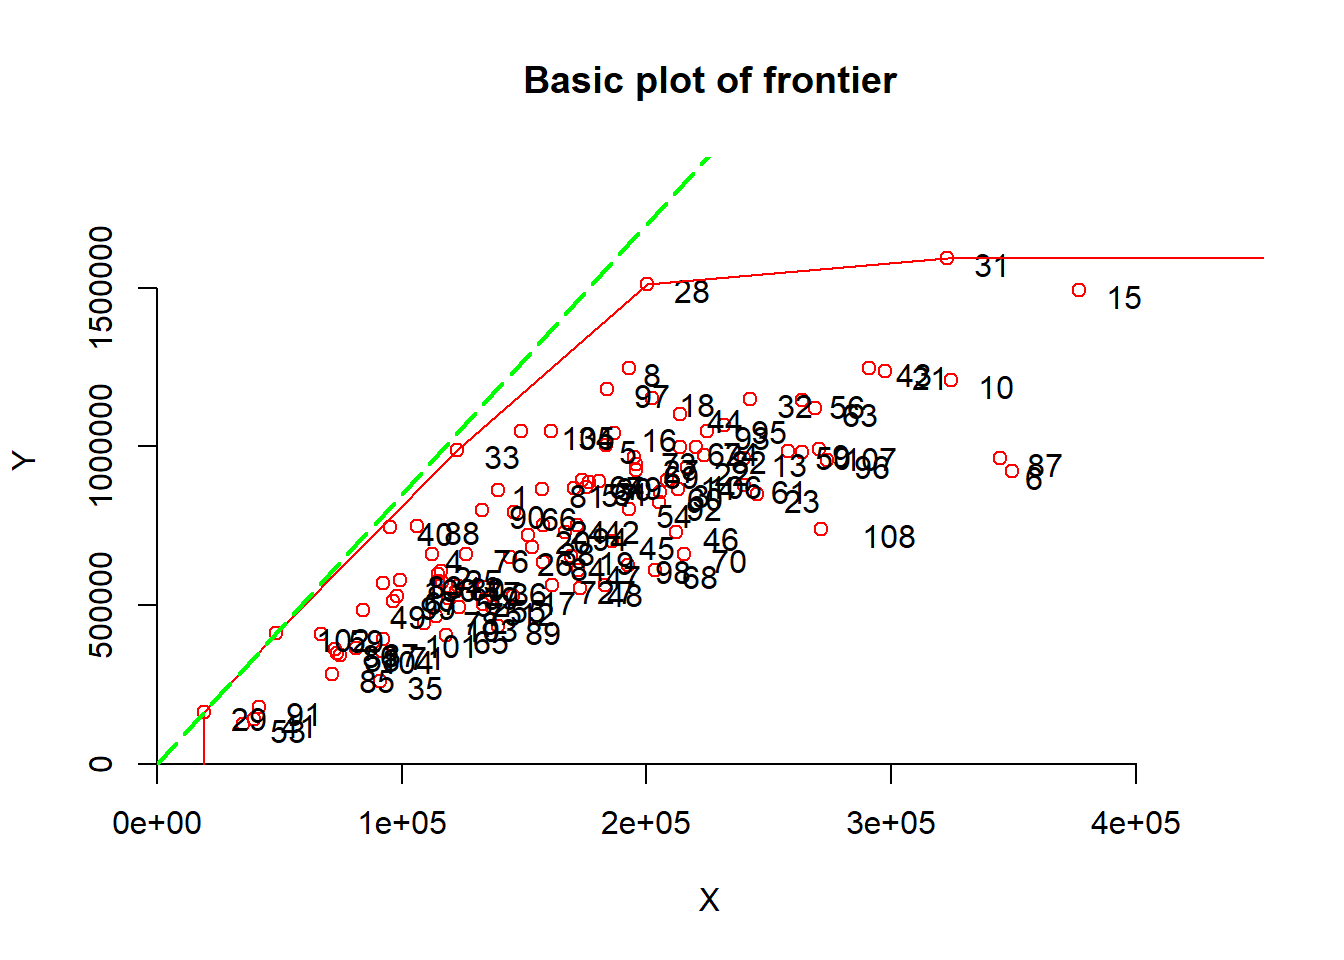
\includegraphics{DEA_notebook_files/figure-latex/unnamed-chunk-11-1.pdf}

Conclusion\\
The number of Farm that produce milk efficiently are still lower than
the inefficient one. There are only 16 farms that produce milk
efficiently, while other 92 farms still produce milk inefficiently. To
achieve efficiency, farm can reduce its input which are energy expenses
and veterinary expenses but there is no need to reduce the number of
cows because it does not make sense to reduce the cows unless they die.

\end{document}
